%%%%%%%%%%%%%%%%
%PARTS REMOVED
%%%%%%%%%%%%%%%%



Solution: 

This can be reached by the entities through the C2 Approach agility and C2 Maneuver Agility, that will combine entities' configuration and coordination in order to adapt themselves for the purpose of further keep in action and quality levels. C2 Approach Agility highlights the ability of a C2 approach, e.g., edge, coordinated, collaborative, de-conflicted or conflicted, to deal with the new context. On the other hand, C2 Maneuver Agility indicates the capacity of the system to change C2 approach in response to the new circumstance. 




Motivation:

Real scenarios with the application of C2 concepts assume a large scale resources consumption, e.g., entities. With that, experiments execution can be extremely expensive and unfeasible. Based on this, our study focuses on application and analysis of results and behaviors in a software simulated environment. Such simulated environments allow us to test a wider range of possibilities and to validate models that translate the behavior of the entities involved in the process. Simulation is widely used to evaluate C2 scenarios, e.g., war games for training and description made by~\cite{Mason2001}. In our case, we are using a custom implementation based on agents to create dynamic scenarios with Unmanned Aerial Vehicle (UAV) similar to what was presented by \cite{Schwarzrock2017} and \cite{UAV01}.




Background:

present the simulator architecture implemented with RePast Symphony~\citep{ABAR201713}




Formulas:

%A valid configuration of a member, resulted from a set of features activated, can be represented as:

\begin{equation}
    \label{eq:prop7}
    c \models t = \exists F' \subseteq F \bullet (c \in P(F')) \land (\mathcal{R}(F', t))
\end{equation}

%, where $\mathcal{R}$ correlates the features $F'$ to the task $t$ indicating their compatibility and their capability to perform the task.


%%%%%%%
Robustness: the ability of keeping the effectiveness level across different missions and circumstances. This effectiveness is the indicator to measure the C2 System's robustness and it is a challenge when we have a complex scenario involving many variables, e.g., threat or environment changes. Different contexts allow the suitable system's robustness measurement.

Resilience: The capability of recovering after some issue or damage. It looks for a stabilization after something that causes perturbation. i.e., onboard component damage or environment perturbation. To measure it, it is required to create stress situations to force some adaptation to the new context. It's correlated with responsiveness and flexibility.

Responsiveness: it is the C2 System ability to act or react according to some context change in a timely manner. There is no unique optimal response and it depends on the resources and circumstances. However it needs to occur within reasonable time frame.

Flexibility: it is the capability of the C2 System to act in different ways to achieve the success. The identification of different paths of execution shows the flexibility level of the system. All these possible paths allow the C2 System to obtain suitable outcomes using the most suitable execution line according to the circumstances.However, the system must have the capability of processing to foresee results in different paths execution to chose the most suitable.

Adaptability: The capability of the system to change its organization or work process to become compatible with the new circumstance. It collaborates with the flexibility and responsiveness. Changes in the network structure are an example of adaptation to obtain different level of information sharing to be suitable to a new circumstance.

\% of successful tasks - effectiveness
Number of reconfigurations - reconfigurations
Number of maneuvers - adaptations

%%%%%%%%%%%%%%%%%%%%%%%%%%%%%%%%%%%%%%%%%%%%%%%%%%%%%%

\begin{figure}[H]
    \centering
    \scalebox{.5}{

\tikzset{every picture/.style={line width=0.75pt}} %set default line width to 0.75pt        

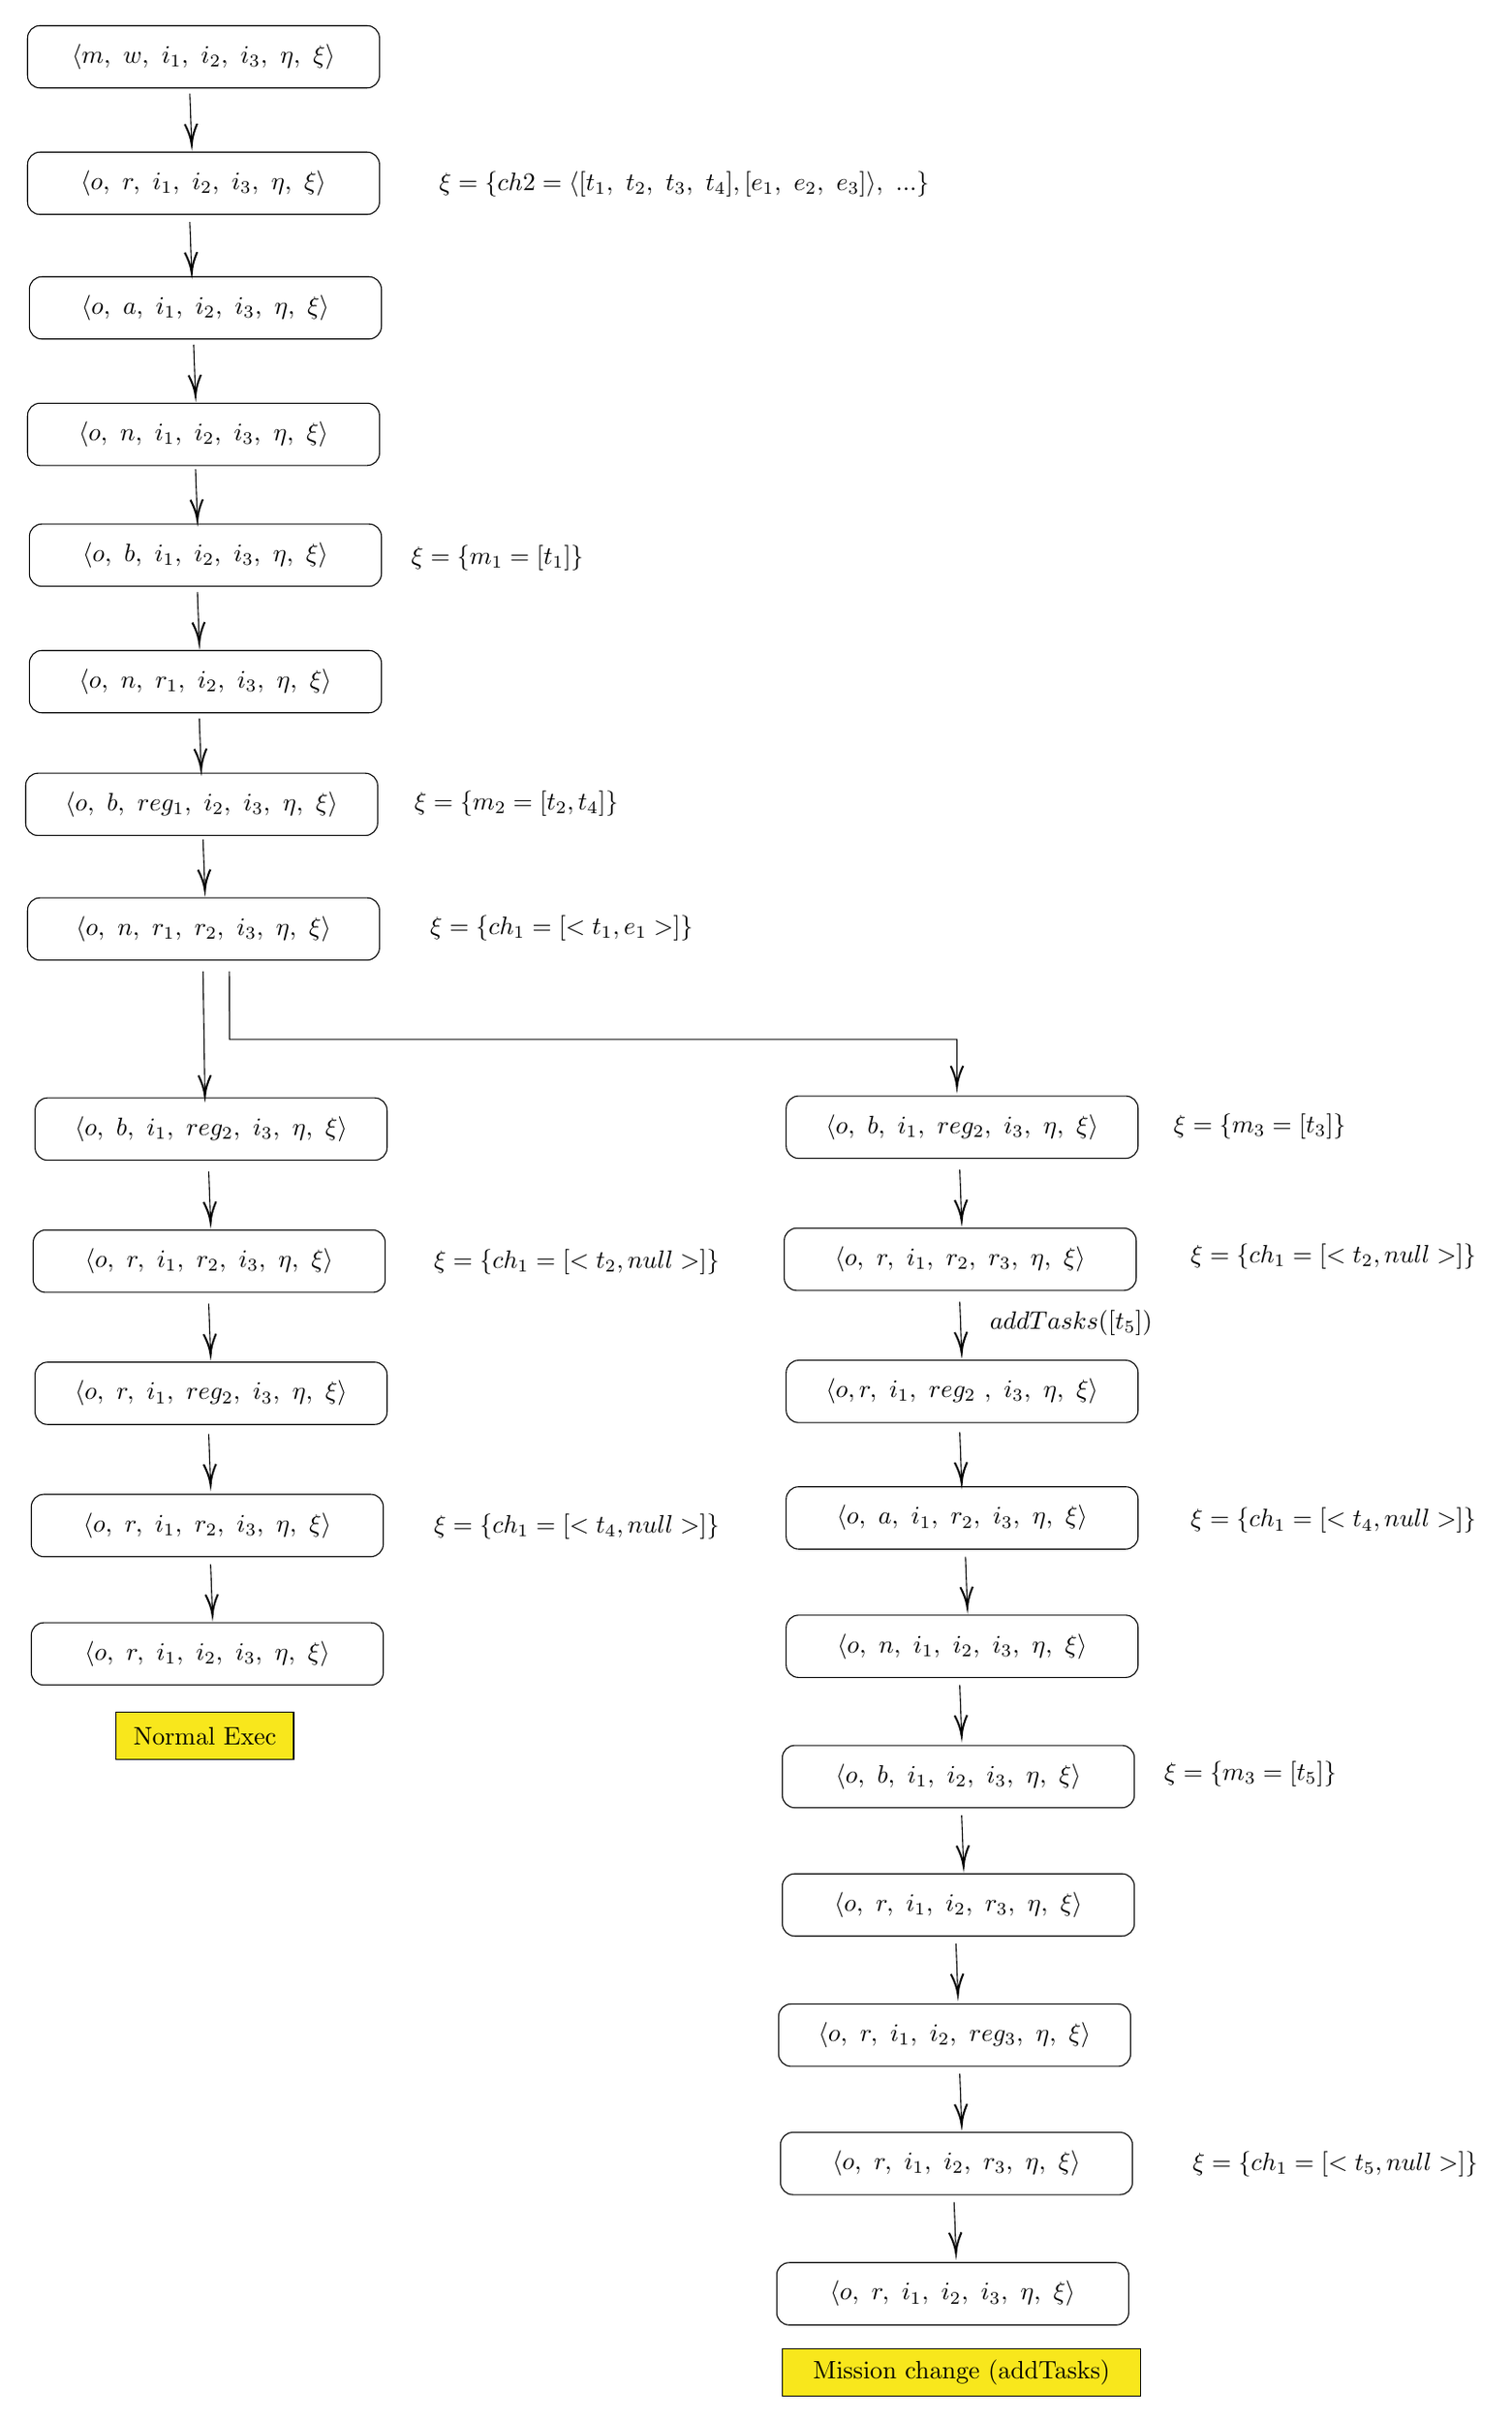
\begin{tikzpicture}[x=0.75pt,y=0.75pt,yscale=-1,xscale=1]
%uncomment if require: \path (0,1284); %set diagram left start at 0, and has height of 1284

%Rounded Rect [id:dp9048297129007524] 
\draw   (19,13.6) .. controls (19,9.95) and (21.95,7) .. (25.6,7) -- (198.9,7) .. controls (202.55,7) and (205.5,9.95) .. (205.5,13.6) -- (205.5,33.4) .. controls (205.5,37.05) and (202.55,40) .. (198.9,40) -- (25.6,40) .. controls (21.95,40) and (19,37.05) .. (19,33.4) -- cycle ;
%Rounded Rect [id:dp8152798292363221] 
\draw   (19,80.6) .. controls (19,76.95) and (21.95,74) .. (25.6,74) -- (198.9,74) .. controls (202.55,74) and (205.5,76.95) .. (205.5,80.6) -- (205.5,100.4) .. controls (205.5,104.05) and (202.55,107) .. (198.9,107) -- (25.6,107) .. controls (21.95,107) and (19,104.05) .. (19,100.4) -- cycle ;
%Rounded Rect [id:dp2611238064001401] 
\draw   (20,146.6) .. controls (20,142.95) and (22.95,140) .. (26.6,140) -- (199.9,140) .. controls (203.55,140) and (206.5,142.95) .. (206.5,146.6) -- (206.5,166.4) .. controls (206.5,170.05) and (203.55,173) .. (199.9,173) -- (26.6,173) .. controls (22.95,173) and (20,170.05) .. (20,166.4) -- cycle ;
%Rounded Rect [id:dp5474323622335151] 
\draw   (19,213.6) .. controls (19,209.95) and (21.95,207) .. (25.6,207) -- (198.9,207) .. controls (202.55,207) and (205.5,209.95) .. (205.5,213.6) -- (205.5,233.4) .. controls (205.5,237.05) and (202.55,240) .. (198.9,240) -- (25.6,240) .. controls (21.95,240) and (19,237.05) .. (19,233.4) -- cycle ;
%Rounded Rect [id:dp617967347556163] 
\draw   (20,277.6) .. controls (20,273.95) and (22.95,271) .. (26.6,271) -- (199.9,271) .. controls (203.55,271) and (206.5,273.95) .. (206.5,277.6) -- (206.5,297.4) .. controls (206.5,301.05) and (203.55,304) .. (199.9,304) -- (26.6,304) .. controls (22.95,304) and (20,301.05) .. (20,297.4) -- cycle ;
%Rounded Rect [id:dp6526355611328125] 
\draw   (20,344.6) .. controls (20,340.95) and (22.95,338) .. (26.6,338) -- (199.9,338) .. controls (203.55,338) and (206.5,340.95) .. (206.5,344.6) -- (206.5,364.4) .. controls (206.5,368.05) and (203.55,371) .. (199.9,371) -- (26.6,371) .. controls (22.95,371) and (20,368.05) .. (20,364.4) -- cycle ;
%Rounded Rect [id:dp6698610095556133] 
\draw   (18,409.6) .. controls (18,405.95) and (20.95,403) .. (24.6,403) -- (197.9,403) .. controls (201.55,403) and (204.5,405.95) .. (204.5,409.6) -- (204.5,429.4) .. controls (204.5,433.05) and (201.55,436) .. (197.9,436) -- (24.6,436) .. controls (20.95,436) and (18,433.05) .. (18,429.4) -- cycle ;
%Rounded Rect [id:dp9742586895494759] 
\draw   (19,475.6) .. controls (19,471.95) and (21.95,469) .. (25.6,469) -- (198.9,469) .. controls (202.55,469) and (205.5,471.95) .. (205.5,475.6) -- (205.5,495.4) .. controls (205.5,499.05) and (202.55,502) .. (198.9,502) -- (25.6,502) .. controls (21.95,502) and (19,499.05) .. (19,495.4) -- cycle ;
%Rounded Rect [id:dp34832491140564725] 
\draw   (23,581.6) .. controls (23,577.95) and (25.95,575) .. (29.6,575) -- (202.9,575) .. controls (206.55,575) and (209.5,577.95) .. (209.5,581.6) -- (209.5,601.4) .. controls (209.5,605.05) and (206.55,608) .. (202.9,608) -- (29.6,608) .. controls (25.95,608) and (23,605.05) .. (23,601.4) -- cycle ;
%Rounded Rect [id:dp07632153248409779] 
\draw   (22,651.6) .. controls (22,647.95) and (24.95,645) .. (28.6,645) -- (201.9,645) .. controls (205.55,645) and (208.5,647.95) .. (208.5,651.6) -- (208.5,671.4) .. controls (208.5,675.05) and (205.55,678) .. (201.9,678) -- (28.6,678) .. controls (24.95,678) and (22,675.05) .. (22,671.4) -- cycle ;
%Rounded Rect [id:dp38638906596830014] 
\draw   (23,721.6) .. controls (23,717.95) and (25.95,715) .. (29.6,715) -- (202.9,715) .. controls (206.55,715) and (209.5,717.95) .. (209.5,721.6) -- (209.5,741.4) .. controls (209.5,745.05) and (206.55,748) .. (202.9,748) -- (29.6,748) .. controls (25.95,748) and (23,745.05) .. (23,741.4) -- cycle ;
%Rounded Rect [id:dp2961818663412775] 
\draw   (21,791.6) .. controls (21,787.95) and (23.95,785) .. (27.6,785) -- (200.9,785) .. controls (204.55,785) and (207.5,787.95) .. (207.5,791.6) -- (207.5,811.4) .. controls (207.5,815.05) and (204.55,818) .. (200.9,818) -- (27.6,818) .. controls (23.95,818) and (21,815.05) .. (21,811.4) -- cycle ;
%Rounded Rect [id:dp1419509373702863] 
\draw   (21,859.6) .. controls (21,855.95) and (23.95,853) .. (27.6,853) -- (200.9,853) .. controls (204.55,853) and (207.5,855.95) .. (207.5,859.6) -- (207.5,879.4) .. controls (207.5,883.05) and (204.55,886) .. (200.9,886) -- (27.6,886) .. controls (23.95,886) and (21,883.05) .. (21,879.4) -- cycle ;
%Straight Lines [id:da25623652531692265] 
\draw    (105,43) -- (105.93,68) ;
\draw [shift={(106,70)}, rotate = 267.88] [color={rgb, 255:red, 0; green, 0; blue, 0 }  ][line width=0.75]    (10.93,-3.29) .. controls (6.95,-1.4) and (3.31,-0.3) .. (0,0) .. controls (3.31,0.3) and (6.95,1.4) .. (10.93,3.29)   ;
%Straight Lines [id:da9454848916406987] 
\draw    (105,111) -- (105.93,136) ;
\draw [shift={(106,138)}, rotate = 267.88] [color={rgb, 255:red, 0; green, 0; blue, 0 }  ][line width=0.75]    (10.93,-3.29) .. controls (6.95,-1.4) and (3.31,-0.3) .. (0,0) .. controls (3.31,0.3) and (6.95,1.4) .. (10.93,3.29)   ;
%Straight Lines [id:da9308850791504091] 
\draw    (107,176) -- (107.93,201) ;
\draw [shift={(108,203)}, rotate = 267.88] [color={rgb, 255:red, 0; green, 0; blue, 0 }  ][line width=0.75]    (10.93,-3.29) .. controls (6.95,-1.4) and (3.31,-0.3) .. (0,0) .. controls (3.31,0.3) and (6.95,1.4) .. (10.93,3.29)   ;
%Straight Lines [id:da6987828125639035] 
\draw    (108,242) -- (108.93,267) ;
\draw [shift={(109,269)}, rotate = 267.88] [color={rgb, 255:red, 0; green, 0; blue, 0 }  ][line width=0.75]    (10.93,-3.29) .. controls (6.95,-1.4) and (3.31,-0.3) .. (0,0) .. controls (3.31,0.3) and (6.95,1.4) .. (10.93,3.29)   ;
%Straight Lines [id:da38465000460546606] 
\draw    (109,307) -- (109.93,332) ;
\draw [shift={(110,334)}, rotate = 267.88] [color={rgb, 255:red, 0; green, 0; blue, 0 }  ][line width=0.75]    (10.93,-3.29) .. controls (6.95,-1.4) and (3.31,-0.3) .. (0,0) .. controls (3.31,0.3) and (6.95,1.4) .. (10.93,3.29)   ;
%Straight Lines [id:da7402304756808019] 
\draw    (110,374) -- (110.93,399) ;
\draw [shift={(111,401)}, rotate = 267.88] [color={rgb, 255:red, 0; green, 0; blue, 0 }  ][line width=0.75]    (10.93,-3.29) .. controls (6.95,-1.4) and (3.31,-0.3) .. (0,0) .. controls (3.31,0.3) and (6.95,1.4) .. (10.93,3.29)   ;
%Straight Lines [id:da32843301316145035] 
\draw    (112,438) -- (112.93,463) ;
\draw [shift={(113,465)}, rotate = 267.88] [color={rgb, 255:red, 0; green, 0; blue, 0 }  ][line width=0.75]    (10.93,-3.29) .. controls (6.95,-1.4) and (3.31,-0.3) .. (0,0) .. controls (3.31,0.3) and (6.95,1.4) .. (10.93,3.29)   ;
%Straight Lines [id:da33931279270538006] 
\draw    (112,508) -- (112.97,572) ;
\draw [shift={(113,574)}, rotate = 269.13] [color={rgb, 255:red, 0; green, 0; blue, 0 }  ][line width=0.75]    (10.93,-3.29) .. controls (6.95,-1.4) and (3.31,-0.3) .. (0,0) .. controls (3.31,0.3) and (6.95,1.4) .. (10.93,3.29)   ;
%Straight Lines [id:da4793309632596934] 
\draw    (115,614) -- (115.93,639) ;
\draw [shift={(116,641)}, rotate = 267.88] [color={rgb, 255:red, 0; green, 0; blue, 0 }  ][line width=0.75]    (10.93,-3.29) .. controls (6.95,-1.4) and (3.31,-0.3) .. (0,0) .. controls (3.31,0.3) and (6.95,1.4) .. (10.93,3.29)   ;
%Straight Lines [id:da7517013161282193] 
\draw    (115,684) -- (115.93,709) ;
\draw [shift={(116,711)}, rotate = 267.88] [color={rgb, 255:red, 0; green, 0; blue, 0 }  ][line width=0.75]    (10.93,-3.29) .. controls (6.95,-1.4) and (3.31,-0.3) .. (0,0) .. controls (3.31,0.3) and (6.95,1.4) .. (10.93,3.29)   ;
%Straight Lines [id:da06264248753342316] 
\draw    (115,753) -- (115.93,778) ;
\draw [shift={(116,780)}, rotate = 267.88] [color={rgb, 255:red, 0; green, 0; blue, 0 }  ][line width=0.75]    (10.93,-3.29) .. controls (6.95,-1.4) and (3.31,-0.3) .. (0,0) .. controls (3.31,0.3) and (6.95,1.4) .. (10.93,3.29)   ;
%Straight Lines [id:da8026456818678067] 
\draw    (116,822) -- (116.93,847) ;
\draw [shift={(117,849)}, rotate = 267.88] [color={rgb, 255:red, 0; green, 0; blue, 0 }  ][line width=0.75]    (10.93,-3.29) .. controls (6.95,-1.4) and (3.31,-0.3) .. (0,0) .. controls (3.31,0.3) and (6.95,1.4) .. (10.93,3.29)   ;
%Straight Lines [id:da5908935857761284] 
\draw    (125.9,508) -- (126,544) -- (511.5,544) -- (511.5,567) ;
\draw [shift={(511.5,569)}, rotate = 270] [color={rgb, 255:red, 0; green, 0; blue, 0 }  ][line width=0.75]    (10.93,-3.29) .. controls (6.95,-1.4) and (3.31,-0.3) .. (0,0) .. controls (3.31,0.3) and (6.95,1.4) .. (10.93,3.29)   ;
%Rounded Rect [id:dp5235637984819839] 
\draw   (421,580.6) .. controls (421,576.95) and (423.95,574) .. (427.6,574) -- (600.9,574) .. controls (604.55,574) and (607.5,576.95) .. (607.5,580.6) -- (607.5,600.4) .. controls (607.5,604.05) and (604.55,607) .. (600.9,607) -- (427.6,607) .. controls (423.95,607) and (421,604.05) .. (421,600.4) -- cycle ;
%Rounded Rect [id:dp6388096895962524] 
\draw   (420,650.6) .. controls (420,646.95) and (422.95,644) .. (426.6,644) -- (599.9,644) .. controls (603.55,644) and (606.5,646.95) .. (606.5,650.6) -- (606.5,670.4) .. controls (606.5,674.05) and (603.55,677) .. (599.9,677) -- (426.6,677) .. controls (422.95,677) and (420,674.05) .. (420,670.4) -- cycle ;
%Rounded Rect [id:dp5869997611694289] 
\draw   (421,720.6) .. controls (421,716.95) and (423.95,714) .. (427.6,714) -- (600.9,714) .. controls (604.55,714) and (607.5,716.95) .. (607.5,720.6) -- (607.5,740.4) .. controls (607.5,744.05) and (604.55,747) .. (600.9,747) -- (427.6,747) .. controls (423.95,747) and (421,744.05) .. (421,740.4) -- cycle ;
%Rounded Rect [id:dp022314564452097563] 
\draw   (419,924.6) .. controls (419,920.95) and (421.95,918) .. (425.6,918) -- (598.9,918) .. controls (602.55,918) and (605.5,920.95) .. (605.5,924.6) -- (605.5,944.4) .. controls (605.5,948.05) and (602.55,951) .. (598.9,951) -- (425.6,951) .. controls (421.95,951) and (419,948.05) .. (419,944.4) -- cycle ;
%Straight Lines [id:da8224843419739402] 
\draw    (513,613) -- (513.93,638) ;
\draw [shift={(514,640)}, rotate = 267.88] [color={rgb, 255:red, 0; green, 0; blue, 0 }  ][line width=0.75]    (10.93,-3.29) .. controls (6.95,-1.4) and (3.31,-0.3) .. (0,0) .. controls (3.31,0.3) and (6.95,1.4) .. (10.93,3.29)   ;
%Straight Lines [id:da009923741291622101] 
\draw    (513,683) -- (513.93,708) ;
\draw [shift={(514,710)}, rotate = 267.88] [color={rgb, 255:red, 0; green, 0; blue, 0 }  ][line width=0.75]    (10.93,-3.29) .. controls (6.95,-1.4) and (3.31,-0.3) .. (0,0) .. controls (3.31,0.3) and (6.95,1.4) .. (10.93,3.29)   ;
%Straight Lines [id:da9146101004501517] 
\draw    (513,752) -- (513.93,777) ;
\draw [shift={(514,779)}, rotate = 267.88] [color={rgb, 255:red, 0; green, 0; blue, 0 }  ][line width=0.75]    (10.93,-3.29) .. controls (6.95,-1.4) and (3.31,-0.3) .. (0,0) .. controls (3.31,0.3) and (6.95,1.4) .. (10.93,3.29)   ;
%Rounded Rect [id:dp7814253079901161] 
\draw   (421,787.6) .. controls (421,783.95) and (423.95,781) .. (427.6,781) -- (600.9,781) .. controls (604.55,781) and (607.5,783.95) .. (607.5,787.6) -- (607.5,807.4) .. controls (607.5,811.05) and (604.55,814) .. (600.9,814) -- (427.6,814) .. controls (423.95,814) and (421,811.05) .. (421,807.4) -- cycle ;
%Rounded Rect [id:dp305019935650948] 
\draw   (421,855.6) .. controls (421,851.95) and (423.95,849) .. (427.6,849) -- (600.9,849) .. controls (604.55,849) and (607.5,851.95) .. (607.5,855.6) -- (607.5,875.4) .. controls (607.5,879.05) and (604.55,882) .. (600.9,882) -- (427.6,882) .. controls (423.95,882) and (421,879.05) .. (421,875.4) -- cycle ;
%Straight Lines [id:da8679776548477948] 
\draw    (516,818) -- (516.93,843) ;
\draw [shift={(517,845)}, rotate = 267.88] [color={rgb, 255:red, 0; green, 0; blue, 0 }  ][line width=0.75]    (10.93,-3.29) .. controls (6.95,-1.4) and (3.31,-0.3) .. (0,0) .. controls (3.31,0.3) and (6.95,1.4) .. (10.93,3.29)   ;
%Straight Lines [id:da12004671848417836] 
\draw    (513,886) -- (513.93,911) ;
\draw [shift={(514,913)}, rotate = 267.88] [color={rgb, 255:red, 0; green, 0; blue, 0 }  ][line width=0.75]    (10.93,-3.29) .. controls (6.95,-1.4) and (3.31,-0.3) .. (0,0) .. controls (3.31,0.3) and (6.95,1.4) .. (10.93,3.29)   ;
%Rounded Rect [id:dp5816939761339539] 
\draw   (417,1061.6) .. controls (417,1057.95) and (419.95,1055) .. (423.6,1055) -- (596.9,1055) .. controls (600.55,1055) and (603.5,1057.95) .. (603.5,1061.6) -- (603.5,1081.4) .. controls (603.5,1085.05) and (600.55,1088) .. (596.9,1088) -- (423.6,1088) .. controls (419.95,1088) and (417,1085.05) .. (417,1081.4) -- cycle ;
%Rounded Rect [id:dp7556879043835839] 
\draw   (419,992.6) .. controls (419,988.95) and (421.95,986) .. (425.6,986) -- (598.9,986) .. controls (602.55,986) and (605.5,988.95) .. (605.5,992.6) -- (605.5,1012.4) .. controls (605.5,1016.05) and (602.55,1019) .. (598.9,1019) -- (425.6,1019) .. controls (421.95,1019) and (419,1016.05) .. (419,1012.4) -- cycle ;
%Straight Lines [id:da9188847600899491] 
\draw    (514,955) -- (514.93,980) ;
\draw [shift={(515,982)}, rotate = 267.88] [color={rgb, 255:red, 0; green, 0; blue, 0 }  ][line width=0.75]    (10.93,-3.29) .. controls (6.95,-1.4) and (3.31,-0.3) .. (0,0) .. controls (3.31,0.3) and (6.95,1.4) .. (10.93,3.29)   ;
%Straight Lines [id:da0007997355672678674] 
\draw    (511,1023) -- (511.93,1048) ;
\draw [shift={(512,1050)}, rotate = 267.88] [color={rgb, 255:red, 0; green, 0; blue, 0 }  ][line width=0.75]    (10.93,-3.29) .. controls (6.95,-1.4) and (3.31,-0.3) .. (0,0) .. controls (3.31,0.3) and (6.95,1.4) .. (10.93,3.29)   ;
%Rounded Rect [id:dp22073158285645345] 
\draw   (416,1198.6) .. controls (416,1194.95) and (418.95,1192) .. (422.6,1192) -- (595.9,1192) .. controls (599.55,1192) and (602.5,1194.95) .. (602.5,1198.6) -- (602.5,1218.4) .. controls (602.5,1222.05) and (599.55,1225) .. (595.9,1225) -- (422.6,1225) .. controls (418.95,1225) and (416,1222.05) .. (416,1218.4) -- cycle ;
%Rounded Rect [id:dp8497689490526584] 
\draw   (418,1129.6) .. controls (418,1125.95) and (420.95,1123) .. (424.6,1123) -- (597.9,1123) .. controls (601.55,1123) and (604.5,1125.95) .. (604.5,1129.6) -- (604.5,1149.4) .. controls (604.5,1153.05) and (601.55,1156) .. (597.9,1156) -- (424.6,1156) .. controls (420.95,1156) and (418,1153.05) .. (418,1149.4) -- cycle ;
%Straight Lines [id:da86292810142037] 
\draw    (513,1092) -- (513.93,1117) ;
\draw [shift={(514,1119)}, rotate = 267.88] [color={rgb, 255:red, 0; green, 0; blue, 0 }  ][line width=0.75]    (10.93,-3.29) .. controls (6.95,-1.4) and (3.31,-0.3) .. (0,0) .. controls (3.31,0.3) and (6.95,1.4) .. (10.93,3.29)   ;
%Straight Lines [id:da6078003611560379] 
\draw    (510,1160) -- (510.93,1185) ;
\draw [shift={(511,1187)}, rotate = 267.88] [color={rgb, 255:red, 0; green, 0; blue, 0 }  ][line width=0.75]    (10.93,-3.29) .. controls (6.95,-1.4) and (3.31,-0.3) .. (0,0) .. controls (3.31,0.3) and (6.95,1.4) .. (10.93,3.29)   ;

% Text Node
\draw (112.25,23.5) node    {$\langle m,\ w,\ i_{1} ,\ i_{2} ,\ i_{3} ,\ \eta ,\ \xi \rangle $};
% Text Node
\draw (112.25,90.5) node    {$\langle o,\ r,\ i_{1} ,\ i_{2} ,\ i_{3} ,\ \eta ,\ \xi \rangle $};
% Text Node
\draw (367,91) node    {$\xi =\{ch2=\langle [ t_{1} ,\ t_{2} ,\ t_{3} ,\ t_{4}] ,[ e_{1} ,\textcolor[rgb]{0,0,0}{\ e}\textcolor[rgb]{0,0,0}{_{2}} ,\ e_{3}] \rangle ,\ ...\}$};
% Text Node
\draw (113.25,156.5) node    {$\langle o,\ a,\ i_{1} ,\ i_{2} ,\ i_{3} ,\ \eta ,\ \xi \rangle $};
% Text Node
\draw (112.25,223.5) node    {$\langle o,\ n,\ i_{1} ,\ i_{2} ,\ i_{3} ,\ \eta ,\ \xi \rangle $};
% Text Node
\draw (113.25,287.5) node    {$\langle o,\ b,\ i_{1} ,\ i_{2} ,\ i_{3} ,\ \eta ,\ \xi \rangle $};
% Text Node
\draw (268,289) node    {$\xi =\{m_{1} =[ t_{1}]\}$};
% Text Node
\draw (113.25,354.5) node    {$\langle o,\ n,\ r_{1} ,\ i_{2} ,\ i_{3} ,\ \eta ,\ \xi \rangle $};
% Text Node
\draw (111.25,419.5) node    {$\langle o,\ b,\ reg_{1} ,\ i_{2} ,\ i_{3} ,\ \eta ,\ \xi \rangle $};
% Text Node
\draw (278,419) node    {$\xi =\{m_{2} =[\textcolor[rgb]{0,0,0}{t}\textcolor[rgb]{0,0,0}{_{2}} ,t_{4}]\}$};
% Text Node
\draw (112.25,485.5) node    {$\langle o,\ n,\ r_{1} ,\ r_{2} ,\ i_{3} ,\ \eta ,\ \xi \rangle $};
% Text Node
\draw (116.25,591.5) node    {$\langle o,\ b,\ i_{1} ,\ reg_{2} ,\ i_{3} ,\ \eta ,\ \xi \rangle $};
% Text Node
\draw (115.25,661.5) node    {$\langle o,\ r,\ i_{1} ,\ r_{2} ,\ i_{3} ,\ \eta ,\ \xi \rangle $};
% Text Node
\draw (116.25,731.5) node    {$\langle o,\ r,\ i_{1} ,\ reg_{2} ,\ i_{3} ,\ \eta ,\ \xi \rangle $};
% Text Node
\draw (114.25,801.5) node    {$\langle o,\ r,\ i_{1} ,\ r_{2} ,\ i_{3} ,\ \eta ,\ \xi \rangle $};
% Text Node
\draw (114.25,869.5) node    {$\langle o,\ r,\ i_{1} ,\ i_{2} ,\ i_{3} ,\ \eta ,\ \xi \rangle $};
% Text Node
\draw (302,485) node    {$\xi =\{ch_{1} =[ < t_{1} ,e_{1}  >]\}$};
% Text Node
\draw (514.25,590.5) node    {$\langle o,\ b,\ i_{1} ,\ reg_{2} ,\ i_{3} ,\ \eta ,\ \xi \rangle $};
% Text Node
\draw (513.25,660.5) node    {$\langle o,\ r,\ i_{1} ,\ r_{2} ,\ r_{3} ,\ \eta ,\ \xi \rangle $};
% Text Node
\draw (514.25,730.5) node    {$\langle o,r,\ i_{1} ,\ reg_{2} \ ,\ i_{3} ,\ \eta ,\ \xi \rangle $};
% Text Node
\draw (512.25,934.5) node    {$\langle o,\ b,\ i_{1} ,\ i_{2} ,\ i_{3} ,\ \eta ,\ \xi \rangle $};
% Text Node
\draw (514.25,797.5) node    {$\langle o,\ a,\ i_{1} ,\ r_{2} ,\ i_{3} ,\ \eta ,\ \xi \rangle $};
% Text Node
\draw (514.25,865.5) node    {$\langle o,\ n,\ i_{1} ,\ i_{2} ,\ i_{3} ,\ \eta ,\ \xi \rangle $};
% Text Node
\draw  [fill={rgb, 255:red, 248; green, 231; blue, 28 }  ,fill opacity=1 ]  (66,900.5) -- (160,900.5) -- (160,925.5) -- (66,925.5) -- cycle  ;
\draw (113,913) node   [align=left] {Normal Exec};
% Text Node
\draw  [fill={rgb, 255:red, 248; green, 231; blue, 28 }  ,fill opacity=1 ]  (419,1237.5) -- (609,1237.5) -- (609,1262.5) -- (419,1262.5) -- cycle  ;
\draw (514,1250) node   [align=left] {Mission change (addTasks)};
% Text Node
\draw (672,590) node    {$\xi =\{m_{3} =[ t_{3}]\}$};
% Text Node
\draw (572,694) node    {$addTasks([ t_{5}])$};
% Text Node
\draw (667,933) node    {$\xi =\{m_{3} =[ t_{5}]\}$};
% Text Node
\draw (510.25,1071.5) node    {$\langle o,\ r,\ i_{1} ,\ i_{2} ,\ reg_{3} ,\ \eta ,\ \xi \rangle $};
% Text Node
\draw (512.25,1002.5) node    {$\langle o,\ r,\ i_{1} ,\ i_{2} ,\ r_{3} ,\ \eta ,\ \xi \rangle $};
% Text Node
\draw (509.25,1208.5) node    {$\langle o,\ r,\ i_{1} ,\ i_{2} ,\ i_{3} ,\ \eta ,\ \xi \rangle $};
% Text Node
\draw (511.25,1139.5) node    {$\langle o,\ r,\ i_{1} ,\ i_{2} ,\ r_{3} ,\ \eta ,\ \xi \rangle $};
% Text Node
\draw (310,662) node    {$\xi =\{ch_{1} =[ < t_{2} ,null >]\}$};
% Text Node
\draw (310,802) node    {$\xi =\{ch_{1} =[ < t_{4} ,null >]\}$};
% Text Node
\draw (711,659) node    {$\xi =\{ch_{1} =[ < t_{2} ,null >]\}$};
% Text Node
\draw (711,799) node    {$\xi =\{ch_{1} =[ < t_{4} ,null >]\}$};
% Text Node
\draw (712,1140) node    {$\xi =\{ch_{1} =[ < t_{5} ,null >]\}$};


\end{tikzpicture}}
    \caption{TS resulted from the CS(Section \ref{sec:channelSystem}) representing a simple scenario combination with 3 members ($e_1, e_2, e_3$) performing EX (initial states $i_1, i_2, i_3$) and C2A (initial state $m$) and TA (initial state $w$) roles. $\eta$ represents internal variables values and $\xi$ shows the values in the channels.}
    \label{fig:TS}
\end{figure}


%%%%%%%%%%%%%%%%%%%%%%%%%%%%%%%%%%%%%%%%%%%%%%%%%%%

METRICS

Some metrics are challenging because of the complex scenario involving many variables and dynamism, e.g., threat or environment changes.


%%%%%%%

Although modern techniques of Model Checking support a large number of states~\citep{MC01}, concurrent systems like ours may suffer from the possibility of states number explosion. \cite{clarkson2014} showed a prototype of Model Checker to QPTL resulted from a transformation of HyperCTL formula. However the checker is impractical for real-world programs and does not provide a timely response in runtime when the system is under a dynamic context. Based on this, our work is an empirical study using simulation-based experiments. 

Even the simulation environment being simpler than real scenarios, it is relevant to a myriad of different domains such as the military~\citep{CC03} and environmental monitoring~\cite{simulation001}. Simulation creates different circumstances to evaluate a solution or product, or to train professionals, reducing the need for resources to create real circumstances. Furthermore, many scenarios occur naturally in virtual environment, such as Network Centric Warfare and telemedicine, making simulations relevant to represent events that occur in virtual world
~\citep{telemedicine01, FRANCE2014, CC01}.



%%%%%%%%%%%%%%%%%%%%%%%%%%%%%%%%%%%%%%%%%%%%%%%%%%%%%%%%%
Related work (removed text)


%The simulation is used in our work to validate the solution proposed and to collect evidence of any important detail from the C2 domain operation. This validation is an element in the flow presented by~\cite{ClaesWohlinPerRuneson2012}. In their work, the validation in academia must to follow some formalization because there is a risk of hide some important aspects due to a technology limitation.

%To operate in scenarios with high level of dynamism, the C2 process needs to be able to give fast response in terms of adaptation, resources application and results level within the time limit to have responsiveness. At this point, \cite{Alberts2011} explored the agility concept and all requirements to obtain it. In our work, the agility is a desired attribute of DSPL adaptation resource, and it guides the C2 modelling. 

%Even being complex and plenty of information, representing the state of the art about C2 Agility, that report did not consider any cost notion. Based on~\cite{Alberts2006} and \cite{C2-20} cited the importance of results measurements as quality evaluation. In real scenarios, the measurements are fundamental to define if the mission is even feasible. 

%%%%%%%%%%%%%%%%%%%%%%%%%%%%%%%%%%%%%%%%%%%%%%%%%%%%%%%%%%%%%%








%CONCLUSION


% Besides, it is important to notice that the set $CtxAct$ can be enriched with more events that represents any kind of context changes explained in Section~\ref{ssec:background_c2}, i.e., self, mission and environment changes.


% \textbf{CS Modelling}:The abstraction used through roles modelling is useful to model a C2 system behaviour giving flexibility to have any quantity of members that perform one or more roles, simultaneously or not. Furthermore, the CS has enabled us to exchange information among different roles running in parallel through their communications structure, so called channels. 

%\textbf{SPL Approaching}: To deal with context changes, the first step is reconfigure the members. To model and implement such behaviour, we considered each member as a Dynamic SPL, i.e., a DSPL, architecture. Such structure is able to adapt themselves in order to activate or deactivate some features and resources onboard to improve its compatibility level with the tasks.





======


 %  \item \textbf{Roles}: The role-based modeling, i.e., using CS, has proven efficient in representing the behavior of the C2 elements and making the model flexible and scalable.
%\end{itemize}
% <> we are assessing the proposed model if it has agility.



======

%these program graphs are used to model roles, i.e., an abstraction of the entities' behavior that is part of a C2 structure. An agent can play one or more instances of a role. Based o this, \citet{agent0010} shows the use of roles as components of agents' implementation for modeling communication and coordination of an agent-based system~\cite{agent1}. These agents can accumulate different types of roles and responsibilities and execute them according to the circumstance~\cite{weyns2019activforms}.